% 
% LaTeX Problem Set Template by Sachin Padmanabhan
% I created this when I was a freshman in CS 103,
% and I continue to use it to this day.
%
% Hope you enjoy!
%
% There may be problems with this template.
% If so, feel free to contact me.
%

% Updated for Summer 2019 by Amy Liu
% Updated for Summer 2020 by Ryan Smith

\documentclass{article}
\usepackage{amsmath}
\usepackage{amssymb}
\usepackage{amsthm}
\usepackage{amssymb}
\usepackage{mathdots}
\usepackage[pdftex]{graphicx}
\usepackage{fancyhdr}
\usepackage[margin=1in]{geometry}
\usepackage{multicol}
\usepackage{bm}
\usepackage{listings}
\PassOptionsToPackage{usenames,dvipsnames}{color}  %% Allow color names
\usepackage{pdfpages}
\usepackage{algpseudocode}
\usepackage{tikz}
\usetikzlibrary{automata,positioning}
\usepackage{enumitem}
\usepackage[T1]{fontenc}
\usepackage{inconsolata}
\usepackage{framed}
\usepackage{wasysym}
\usepackage[thinlines]{easytable}
\usepackage{wrapfig}
\usepackage{hyperref}
\usepackage{mathrsfs}
\usepackage{tabularx} % also loads 'array' package
\newcolumntype{C}{>{\centering\arraybackslash}X} % centered version of 'X' columns
\usepackage{diagbox}

\title{CS 103: Mathematical Foundations of Computing\\Problem Set \#4}
\author{Your Name(s) Here}
\date{\today}

\lhead{Your Name(s) Here}
\chead{Problem Set \#5}
\rhead{\today}
\lfoot{}
\cfoot{CS 103: Mathematical Foundations of Computing --- Summer 2020}
\rfoot{\thepage}

\newcommand{\abs}[1]{\lvert #1 \rvert}
\newcommand{\absfit}[1]{\left\lvert #1 \right\rvert}
\newcommand{\norm}[1]{\left\lVert #1 \right\rVert}
\newcommand{\eval}[3]{\left[#1\right]_{#2}^{#3}}
\renewcommand{\(}{\left(}
\renewcommand{\)}{\right)}
\newcommand{\floor}[1]{\left\lfloor#1\right\rfloor}
\newcommand{\ceil}[1]{\left\lceil#1\right\rceil}
\newcommand{\pd}[1]{\frac{\partial}{\partial #1}}
\newcommand{\inner}[1]{\langle#1\rangle}
\newcommand{\cond}{\bigg|}
\newcommand{\rank}[1]{\mathbf{rank}(#1)}
\newcommand{\range}[1]{\mathbf{range}(#1)}
\newcommand{\nullsp}[1]{\mathbf{null}(#1)}
\newcommand{\repr}[1]{\left\langle#1\right\rangle}
\newcommand\VRule[1][\arrayrulewidth]{\vrule width #1}

\DeclareMathOperator{\Var}{Var}
\DeclareMathOperator{\tr}{tr}
\DeclareMathOperator{\Tr}{\mathbf{Tr}}
\DeclareMathOperator{\diag}{\mathbf{diag}}
\DeclareMathOperator{\dist}{\mathbf{dist}}
\DeclareMathOperator{\prob}{\mathbf{prob}}
\DeclareMathOperator{\dom}{\mathbf{dom}}
\DeclareMathOperator{\E}{\mathbf{E}}
\DeclareMathOperator{\Q}{\mathbb{Q}}
\DeclareMathOperator{\R}{\mathbb{R}}
\DeclareMathOperator{\var}{\mathbf{var}}
\DeclareMathOperator{\quartile}{\mathbf{quartile}}
\DeclareMathOperator{\conv}{\mathbf{conv}}
\DeclareMathOperator{\VC}{VC}
\DeclareMathOperator*{\argmax}{arg\,max}
\DeclareMathOperator*{\argmin}{arg\,min}
\DeclareMathOperator{\Ber}{Bernoulli}
\DeclareMathOperator{\NP}{\mathbf{NP}}
\DeclareMathOperator{\coNP}{\mathbf{coNP}}
\DeclareMathOperator{\TIME}{\mathsf{TIME}}
\DeclareMathOperator{\polytime}{\mathbf{P}}
\DeclareMathOperator{\PH}{\mathbf{PH}}
\DeclareMathOperator{\SIZE}{\mathbf{SIZE}}
\DeclareMathOperator{\ATIME}{\mathbf{ATIME}}
\DeclareMathOperator{\SPACE}{\mathbf{SPACE}}
\DeclareMathOperator{\ASPACE}{\mathbf{ASPACE}}
\DeclareMathOperator{\NSPACE}{\mathbf{NSPACE}}
\DeclareMathOperator{\Z}{\mathbb{Z}}
\DeclareMathOperator{\N}{\mathbb{N}}
\DeclareMathOperator{\EXP}{\mathbf{EXP}}
\DeclareMathOperator{\NEXP}{\mathbf{NEXP}}
\DeclareMathOperator{\NTIME}{\mathbf{NTIME}}
\DeclareMathOperator{\DTIME}{\mathbf{DTIME}}
\DeclareMathOperator{\poly}{poly}
\DeclareMathOperator{\BPP}{\mathbf{BPP}}
\DeclareMathOperator{\ZPP}{\mathbf{ZPP}}
\DeclareMathOperator{\RP}{\mathbf{RP}}
\DeclareMathOperator{\coRP}{\mathbf{coRP}}
\DeclareMathOperator{\BPL}{\mathbf{BPL}}
\DeclareMathOperator{\IP}{\mathbf{IP}}
\DeclareMathOperator{\PSPACE}{\mathbf{PSPACE}}
\DeclareMathOperator{\NPSPACE}{\mathbf{NPSPACE}}
\DeclareMathOperator{\SAT}{\mathsf{SAT}}
\DeclareMathOperator{\NL}{\mathbf{NL}}
\DeclareMathOperator{\PCP}{\mathbf{PCP}}
\DeclareMathOperator{\PP}{\mathbf{PP}}
\DeclareMathOperator{\cost}{cost}
\let\Pr\relax
\DeclareMathOperator*{\Pr}{\mathbf{Pr}}

\definecolor{shadecolor}{gray}{0.9}

\theoremstyle{plain}
\newtheorem*{lem}{Lemma}

\theoremstyle{plain}
\newtheorem*{claim}{Claim}

\theoremstyle{definition}
\newtheorem*{answer}{Answer}

\newtheorem{theorem}{Theorem}[section]
\newtheorem*{thm}{Theorem}
\newtheorem{corollary}{Corollary}[theorem]
\newtheorem{lemma}[theorem]{Lemma}

\renewcommand{\headrulewidth}{0.4pt}
\renewcommand{\footrulewidth}{0.4pt}

\setlength{\parindent}{0pt}

\pagestyle{fancy}

\renewcommand{\thefootnote}{\fnsymbol{footnote}}

% start MZ
\usetikzlibrary{automata,positioning}
\let\oldemptyset\emptyset
\renewcommand{\emptyset}{\text{\O}}
\renewcommand\qedsymbol{$\blacksquare$}
\newenvironment{prf}{{\bfseries Proof.}}{\qedsymbol}
\renewcommand{\emph}[1]{\textit{\textbf{#1}}}
\newcommand{\annotate}[1]{\textit{\textcolor{blue}{#1}}}
\usepackage{stmaryrd}
%\usepackage{minted}
\usepackage{mathtools}
\usepackage{alltt}
\newcommand{\ttt}[1]{\texttt{#1}}
\newcommand{\match}[1]{\textbf{\underline{#1}}}

\begin{document}

\maketitle

\textbf{No checkpoint this week (or any subsequent week!)}

\textbf{All questions due Thursday, July 30th at 11:59PM.} \\

You have an extra week for this problem set since there is a midterm on July 23rd. However, this problem set is longer than normal and includes an extra week of material so you'll definitely want to start to be putting work into it a little earlier than normal. Our goal is for this to be around 1.3-1.5 of a normal problem set.

\textbf{Additionally, some of the questions is on material not covered until much closer to the due date. Try to do problems as we cover the material in class so you don't get overwhelmed!}



Before beginning this problem set, we \emph{strongly} recommend reading over the following handouts:
\begin{itemize}
\item The ``Guide to Induction,'' contains a lot of useful advice about how to approach problems inductively, how to structure inductive proofs, and how to not fall into common inductive traps.
\item The ``Induction Proofwriting Checklist,'' which contains a list of specific things to watch for in your solutions before submitting.
\end{itemize}
As a note on this problem set - normally, you're welcome to use any proof technique you'd like to prove results in this course. On this problem set, we've specifically requested on some problems that you prove a result inductively. For those problems, you should prove those results using induction or complete induction, even if there is another way to prove the result. (If you'd like to use induction in conjunction with other techniques like proof by contradiction or proof by contrapositive, that's perfectly fine.) \\

Note that some of the questions will require you to submit an automata or regular expression you create
via our online editors. Please follow the instructions in the handout to access these tools and submit your work. Some of these tools may not be up and running until we cover the appropriate material in class.
There is no need to copy your constructions back into this written submission as we will look only at your
online submission for grading these questions. \\ 

As always, please feel free to drop by office hours, ask on Campuswire, or email the staff list if you have
any questions. We'd be happy to help out. \\

Good luck, and have fun! 
\pagebreak





\section{Symmetries, Permutations, and Automorphisms}

One of the more beautiful concepts in mathematics is \textit{symmetry}. Chances are that you have some intuitive conception of what ``symmetry'' means, and not just in the binary relation sense. For example, the letter M looks like itself when you look at it in a mirror, and the number 8 looks like itself if you flip it horizontally or rotate it $180^\circ$. \\

Now that we're studying graphs, we can ask what it means for a graph to be symmetric. For example, consider the graph of the  star shown below. This graph has many symmetries -- if you flip it horizontally, or rotate it $72^\circ$, the resulting graph looks identical. But this notion of ``looks identical'' appeals to our human visual system, which, as you've probably experienced, is easily tricked. Is there a way to come up with a more rigorous definition of ``symmetry?'' \\

Let's begin by labeling the nodes of this graph in whatever way we'd like. For convenience, we'll use the numbers 0, 1, 2, 3, and 4, following our star-drawing convention. Now, take the graph shown below and rotate it one fifth of a revolution clockwise, as shown here:

\begin{center}
\begin{minipage}{0.45\textwidth}
\begin{flushright}
\tikzset{every state/.style={inner sep=1pt,minimum size=0pt}}
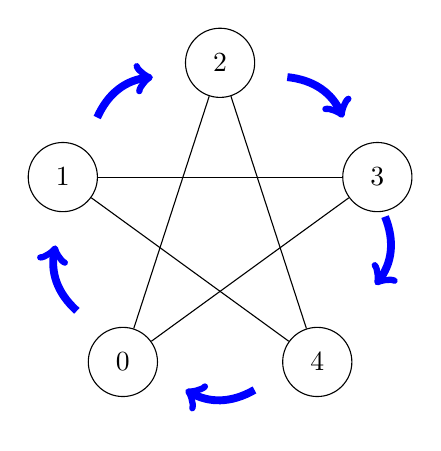
\begin{tikzpicture}[scale=.7,on grid,auto,baseline={(current bounding box.north)}]
  \node[state] (0) at (234:3) {0};
  \node[state] (1) at (162:3) {1};
  \node[state] (2) at (90:3) {2};
  \node[state] (3) at (18:3) {3};
  \node[state] (4) at (306:3) {4};
  \coordinate (a1) at (66:3);
  \coordinate (a2) at (138:3);
  \coordinate (a3) at (210:3);
  \coordinate (a4) at (282:3);
  \coordinate (a5) at (364:3);
  \coordinate (b1) at (42:3);
  \coordinate (b2) at (114:3);
  \coordinate (b3) at (186:3);
  \coordinate (b4) at (258:3);
  \coordinate (b5) at (340:3);
  \path[-] 
    (0) edge node {} (2)
    (2) edge node {} (4)
    (4) edge node {} (1)
    (1) edge node {} (3)
    (3) edge node {} (0);
  \path[->,blue,line width=1mm] 
    (a1) edge [bend left=30] node {} (b1)
    (a2) edge [bend left=30] node {} (b2)
    (a3) edge [bend left=30] node {} (b3)
    (a4) edge [bend left=30] node {} (b4)
    (a5) edge [bend left=30] node {} (b5);
\end{tikzpicture}
\end{flushright}
\end{minipage}
\hfill
\begin{minipage}{0.45\textwidth}
\tikzset{every state/.style={inner sep=1pt,minimum size=0pt}}
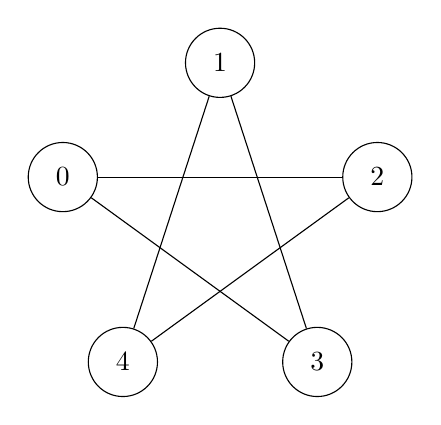
\begin{tikzpicture}[scale=.7,on grid,auto,baseline={(current bounding box.north)}]
  \node[state] (0) at (162:3) {0};
  \node[state] (1) at (90:3) {1};
  \node[state] (2) at (18:3) {2};
  \node[state] (3) at (306:3) {3};
  \node[state] (4) at (234:3) {4};
  \path[-] 
    (0) edge node {} (2)
    (2) edge node {} (4)
    (4) edge node {} (1)
    (1) edge node {} (3)
    (3) edge node {} (0);
\end{tikzpicture}
\end{minipage}
\end{center}

If you'll notice, this operation on the graph corresponds to finding a permutation of the labels on the nodes. Specifically, the node 0 ended up where the node 1 used to be, the node 1 ended up where the node 2 used to be, etc. And hey! We have a way of describing transformations like that.

\begin{enumerate}[label=\roman*.]
    \item Describe the permutation that the above rotation corresponds to using two-line notation. No justification is necessary.
    
    \begin{shaded}
    $$
    \begin{pmatrix}
    	0 & 1 & 2 & 3 & 4 \\
    	1 & 2 & 3 & 4 & 0
    \end{pmatrix}
    $$
    \end{shaded}
\end{enumerate}

\pagebreak
Similarly, let's imagine that we mirror the graph horizontally, as shown here:

\begin{center}
\begin{minipage}{0.45\textwidth}
\begin{flushright}
\tikzset{every state/.style={inner sep=1pt,minimum size=0pt}}
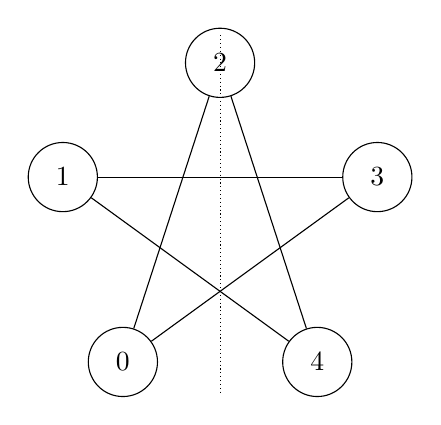
\begin{tikzpicture}[scale=.7,on grid,auto,baseline={(current bounding box.north)}]
  \node[state] (0) at (234:3) {0};
  \node[state] (1) at (162:3) {1};
  \node[state] (2) at (90:3) {2};
  \node[state] (3) at (18:3) {3};
  \node[state] (4) at (306:3) {4};
  \coordinate (a) at (90:3.5);
  \coordinate (b) at (270:3);
  \path[-] 
    (0) edge node {} (2)
    (2) edge node {} (4)
    (4) edge node {} (1)
    (1) edge node {} (3)
    (3) edge node {} (0);
  \path[-,thin,densely dotted]
    (a) edge node {} (b);
\end{tikzpicture}
\end{flushright}
\end{minipage}
\hfill
\begin{minipage}{0.45\textwidth}
\tikzset{every state/.style={inner sep=1pt,minimum size=0pt}}
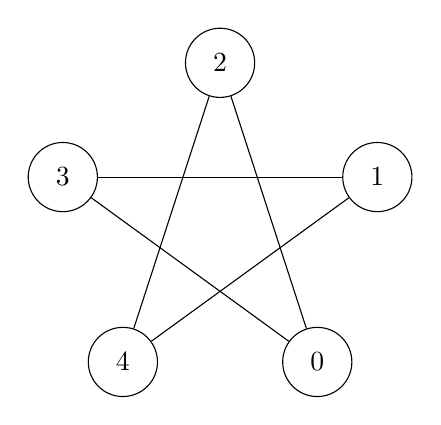
\begin{tikzpicture}[scale=.7,on grid,auto,baseline={(current bounding box.north)}]
  \node[state] (4) at (234:3) {4};
  \node[state] (3) at (162:3) {3};
  \node[state] (2) at (90:3) {2};
  \node[state] (1) at (18:3) {1};
  \node[state] (0) at (306:3) {0};
  \path[-] 
    (0) edge node {} (2)
    (2) edge node {} (4)
    (4) edge node {} (1)
    (1) edge node {} (3)
    (3) edge node {} (0);
\end{tikzpicture}
\end{minipage}
\end{center}

We can similarly think of this as a permutation. For example, node 1 maps to where node 3 used to be.

\begin{enumerate}[resume*]
    \item Describe the permutation that the above mirroring corresponds to using two-line notation. No justification is necessary.
    
    \begin{shaded}
    $$
    \begin{pmatrix}
    	0 & 1 & 2 & 3 & 4 \\
    	4 & 3 & 2 & 1 & 0
    \end{pmatrix}
    $$
    \end{shaded}
\end{enumerate}

There are a number of other symmetries of this graph, and each one of them corresponds to a permutation of the nodes. However, not all node permutations correspond to symmetries. For example, imagine that we permute the nodes as shown here:

\begin{center}
\begin{minipage}{0.45\textwidth}
\begin{flushright}
\tikzset{every state/.style={inner sep=1pt,minimum size=0pt}}
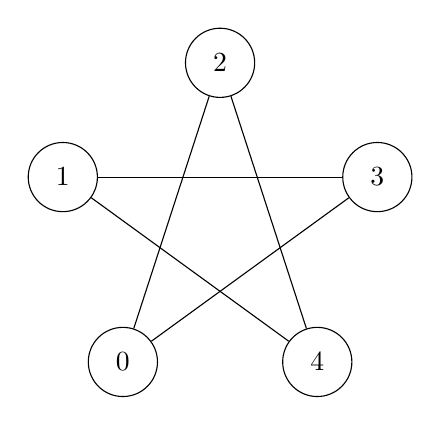
\begin{tikzpicture}[scale=.7,on grid,auto,baseline={(current bounding box.north)}]
  \node[state] (0) at (234:3) {0};
  \node[state] (1) at (162:3) {1};
  \node[state] (2) at (90:3) {2};
  \node[state] (3) at (18:3) {3};
  \node[state] (4) at (306:3) {4};
  \path[-] 
    (0) edge node {} (2)
    (2) edge node {} (4)
    (4) edge node {} (1)
    (1) edge node {} (3)
    (3) edge node {} (0);
\end{tikzpicture}
\end{flushright}
\end{minipage}
\hfill$\xRightarrow{\hphantom{-} ? \hphantom{-}}$\hfill
\begin{minipage}{0.45\textwidth}
\tikzset{every state/.style={inner sep=1pt,minimum size=0pt}}
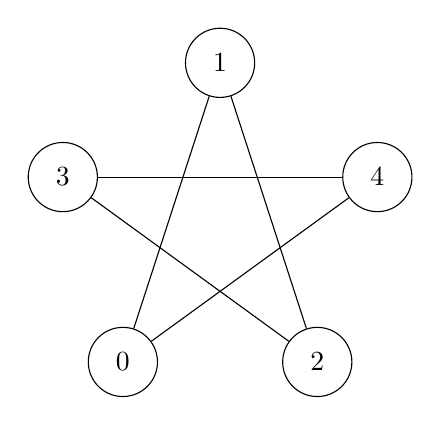
\begin{tikzpicture}[scale=.7,on grid,auto,baseline={(current bounding box.north)}]
  \node[state] (0) at (234:3) {0};
  \node[state] (3) at (162:3) {3};
  \node[state] (1) at (90:3) {1};
  \node[state] (4) at (18:3) {4};
  \node[state] (2) at (306:3) {2};
  \path[-] 
    (0) edge node {} (1)
    (1) edge node {} (2)
    (2) edge node {} (3)
    (3) edge node {} (4)
    (4) edge node {} (0);
\end{tikzpicture}
\end{minipage}
\end{center}

Notice that, in the original graph, nodes 0 and 2 were adjacent, but after permuting the nodes they're no longer adjacent to one another. (Remember that \textit{adjacent} means ``directly linked by an edge;'' contrast this with \textit{connected}, which has a different meaning.) Similarly, in the original graph, nodes 0 and 1 were \textit{not} adjacent, but after applying the permutation they now are. \\

At this point, we've seen some positive examples of cases where we \textit{can} use permutations to model symmetries, along with a negative example of where we \textit{can't} use permutations to model symmetries. The question is, what was special about those original permutations? It's that they have the following property: those permutations keep adjacent nodes adjacent and keep non-adjacent nodes non-adjacent. \\

Formally speaking, let $G = (V, E)$ be a graph. A permutation $\sigma$ of the nodes of $V$ is called an \emph{automorphism} if the following is true about $\sigma$:
$$\forall u \in V. \forall v \in V . (\{u, v\} \in E \iff \{\sigma(u), \sigma(v)\} \in E)$$

The mathematical term ``automorphism'' (``self shape'') might seem really scary here, but it's just a fancy way of pinning down what we've been describing with the term ``symmetry.'' Restating the above in plain English, a permutation is an \emph{automorphism} of $G$ if
\begin{itemize}
    \item any two nodes that are adjacent in $G$ stay adjacent after applying $\sigma$, and
    \item any two nodes that aren't adjacent in $G$ stay nonadjacent after applying $\sigma$.
\end{itemize}

The permutations that you described in parts (i) and (ii) are automorphisms, while the permutation shown above on this page isn't. The rest of this question explores properties of automorphisms.

\begin{enumerate}[resume*]
    \item How many automorphisms does the graph of the above star have? Briefly describe what they are. No formal proof is needed.
    
    \annotate{Use your intuition behind what automorphisms are designed to formalize.}
    
    \begin{shaded}
    Write your answer here.
    \end{shaded}
    
    \item Consider the graph shown below. It has two automorphisms. What are they? Express your answer using two-line notation.

    \begin{center}
    \begin{minipage}{0.5\textwidth}
    \tikzset{every state/.style={inner sep=1pt,minimum size=0pt}}
    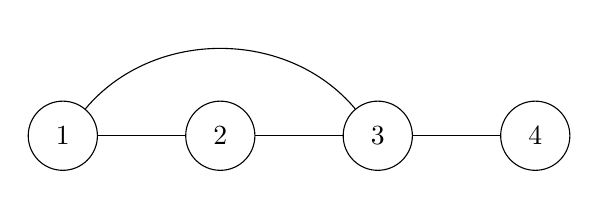
\begin{tikzpicture}[node distance=2cm,on grid,auto,baseline={(current bounding box.north)}]
      \node[state] (1) {1};
      \node[state] (2) [right=of 1] {2};
      \node[state] (3) [right=of 2] {3};
      \node[state] (4) [right=of 3] {4};
      \path[-] 
        (1) edge node {} (2)
        (2) edge node {} (3)
        (3) edge node {} (4)
        (1) edge [bend left=50] node {} (3);
    \end{tikzpicture}
    \end{minipage}
    \end{center}
    
    A graph is just a pair of a set of nodes and a set of edges. We can draw a graph $G = (V, E)$ in two-dimensional space as a collection of circles and lines in lots of different ways. Sometimes, those drawings make it really easy to find symmetries. Sometimes, those drawings make it really hard to find symmetries.
    
    \begin{shaded}
    Write your answer here.
    \end{shaded}
    
\end{enumerate}

To round out our discussion of automorphisms, we'd like you to prove one nice, formal result about them.

\begin{enumerate}[resume*]
    \item Let $G = (V, E)$ be a graph and let $\sigma$ and $\tau$ be two automorphisms of $G$. Prove that $\tau \circ \sigma$ is also an automorphism of $G$.
    
    \annotate{Write out the definition of an automorphism and make a list of what you'll need to show.}
    
    \begin{shaded}
    Provide a proof here.
    \end{shaded}
\end{enumerate}

\pagebreak


\section{Tiling with Triominoes}

A \emph{right triomino} is an L-shaped tile that looks like this: 
\begin{center}

\begin{tikzpicture}[scale=0.65]
\fill[black!25] (0,0) rectangle (2,1);
\fill[black!25] (0,1) rectangle (1,-1);
\draw[very thick] (0,1) -- (2,1);
\draw[very thick] (2,1) -- (2,0);
\draw[very thick] (1,0) -- (2,0);
\draw[very thick] (1,0) -- (1,-1);
\draw[very thick] (0,-1) -- (1,-1);
\draw[very thick] (0,1) -- (0,-1);
\end{tikzpicture}
\end{center}
Suppose you're given a $2^n \times 2^n$ grid of squares and want to tile it with right triominoes by covering the grid with triominoes such that all triominoes are completely on the grid and no triominoes overlap. Here's an attempt to cover an $8 \times 8$ grid with triominoes, which doesn't manage to cover all squares: \\
\begin{center}
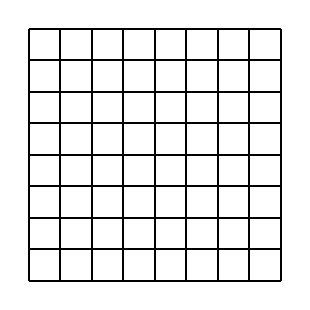
\begin{tikzpicture}[scale=0.4]
\foreach \x in {0,...,8} {
        \draw[thick] (\x, 0) -- (\x, 8);
        \draw[thick] (0, \x) -- (8, \x);
}
\end{tikzpicture}
\hspace{0.8cm}
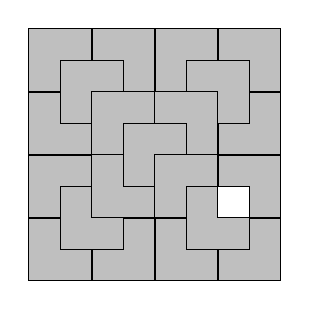
\begin{tikzpicture}[scale=0.4]
\draw [fill=black!25] (0, 0) rectangle (8, 8);
\foreach \x in {1,...,3} {
       \draw[thick] (2*\x, 0) -- (2*\x, 8);
       \draw[thick] (0, 2*\x) -- (8, 2*\x);
}
\draw [fill=black!25] (1, 1) rectangle (3, 3);
\draw [fill=black!25] (1, 5) rectangle (3, 7);
\draw [fill=black!25] (5, 5) rectangle (7, 7);
\draw [fill=black!25] (2, 2) rectangle (4, 4);
\draw [fill=black!25] (2, 4) rectangle (4, 6);
\draw [fill=black!25] (4, 4) rectangle (6, 6);
\draw [fill=black!25] (3, 3) rectangle (5, 5);
\draw [fill=black!25] (4, 2) rectangle (6, 4);
\draw [fill=black!25] (5, 1) rectangle (7, 3);
\draw [fill=white] (6,2) rectangle (7,3);
\end{tikzpicture}
\end{center}

Amazingly, it turns out that it is always possible to tile any $2^n \times 2^n$ grid that's missing exactly one square with right triominoes. It doesn't matter what $n$ is or which square is removed; there is always a solution to the problem. For example, here are all the ways to tile a $4 \times 4$ grid that has a square missing: \\

\begin{center}
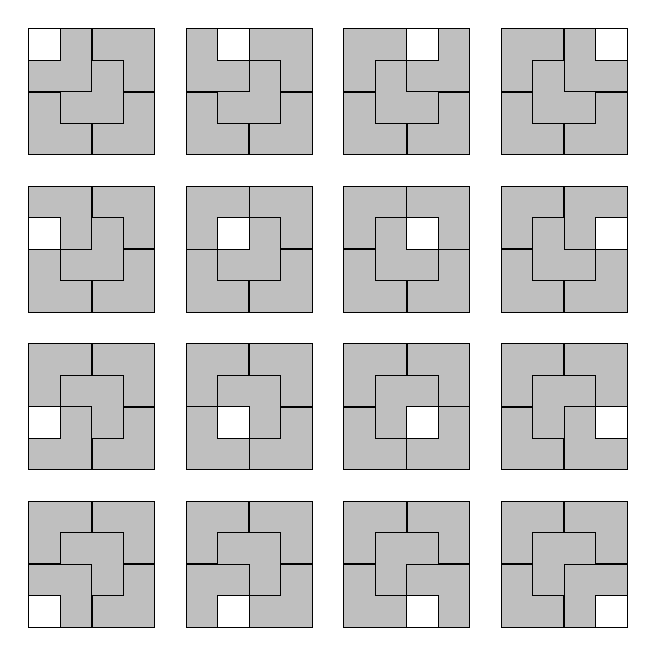
\begin{tikzpicture}[scale=0.4]
\foreach \x in {0,...,3} \foreach \y in {0,...,3} {
        \draw [fill=black!25] (5*\x+1, 5*\y+1) rectangle (5*\x+5, 5*\y+5);
        \draw[thick] (5*\x+3, 5*\y+1) -- (5*\x+3, 5*\y+5);
        \draw[thick] (5*\x+1, 5*\y+3) -- (5*\x+5, 5*\y+3);
        \draw [fill=black!25] (5*\x+2, 5*\y+2) rectangle (5*\x+4, 5*\y+4);
        \draw [fill=white] (6*\x+1, 6*\y+1) rectangle (6*\x+2, 6*\y+2);
}
\foreach \x in {0,...,1} \foreach \y in {0,...,1} {
	\draw [fill=black!25] (5*\x+1, 5*\y+1) rectangle (5*\x+3, 5*\y+3);
	\draw [fill=black!25] (5*\x+1, 5*\y+13) rectangle (5*\x+3, 5*\y+15);
	\draw [fill=black!25] (5*\x+13, 5*\y+1) rectangle (5*\x+15, 5*\y+3);
	\draw [fill=black!25] (5*\x+13, 5*\y+13) rectangle (5*\x+15, 5*\y+15);
}
\foreach \x in {0,...,3} \foreach \y in {0,...,3} {
        \draw [fill=white] (6*\x+1, 6*\y+1) rectangle (6*\x+2, 6*\y+2);
}
\end{tikzpicture}
\end{center}

This question explores why this is the case.

\begin{enumerate}[label*=\roman*.,ref=\roman*]
    \item Prove, by induction, that $4^n - 1$ is a multiple of three for any $n \in \N$ (An integer $n$ is a multiple of three if there is an integer $k$ such that $n = 3k$).
    
    \begin{shaded}
    Provide a proof here.
    \end{shaded}
\end{enumerate}

Any $2^n \times 2^n$ grid missing a square has a number of squares has exactly $4^n - 1$ squares, and so its number of squares is a multiple of three. Although you \textit{can} show that a figure \textit{can't} be tiled with triominoes by showing that its number of squares isn't a multiple of three, you \textit{can't} show that a figure \textit{can} be tiled with triominoes purely by showing that its number of squares is a multiple of three. The arrangement matters. \\

To convince yourself of this, can you think of an example of a grid made of squares where the number of squares \textit{is} a multiple of three, yet the figure cannot be tiled with right triominoes? This shows that your result from part i) is \textit{not} sufficient to prove that any $2^n \times 2^n$ grid that's missing exactly one square can be tiled with right triominoes.

\begin{enumerate}[resume*]
    \item Prove by induction that for any natural number $n$, any $2^n \times 2^n$ grid with any one square removed can be tiled by right triominoes. \\

    \annotate{Before you write this proof, try seeing if you can  find a nice recursive pattern you can follow that will let you fully tile any such board. You should be able to easily tile any $8 \times 8$ chessboard missing a square with right triominoes before you attempt to write up your answer. Once you can do this, formalize your idea in your answer. You may want to think about how to start with a larger board and subdivide it into some number of smaller boards.}
    
    \begin{shaded}
    Provide a proof here.
    \end{shaded}
\end{enumerate}

\pagebreak

\section{The Circle Game}

Here's a game you can play. Suppose that you have a circle with $2n$ arbitrarily-chosen points on its circumference. Of these $2n$ points, $n$ of these points are labeled $+1$, and the remaining $n$ are labeled $-1$. One sample circle with eight points, of which four are labeled $+1$ and four are labeled $-1$, is shown below. \\

Here's the rules of the game. First, choose one of the $2n$ points as your starting point. Then, start moving clockwise around the circle. As you go, you'll pass through some number of $+1$ points and some number of $-1$ points. You lose the game if at any point on your journey you pass through more $-1$ points than $+1$ points. You win the game if you get all the way back around to your starting point without losing. \\

\begin{minipage}[t]{.65\textwidth}
For example, if you started at point A, the game would go like this: 
\begin{center}
\parbox{5cm}{
Start at A: +1. \\
Pass through B: +2.\\
Pass through C: +1.\\
Pass through D: 0.\\
Pass through E: -1. \textit{(You lose.)}
}
\end{center}
If you started at point G, the game would go like this:
\begin{center}
\parbox{5cm}{
Start at G: -1 \textit{(You lose.)}
}
\end{center}
However, if you started at point F, the game would go like this: 
\begin{center}
\parbox{5cm}{
Start at F: +1. \\
Pass through G: 0. \\
Pass through H: +1. \\
Pass through A: +2. \\
Pass through B: +3. \\
Pass through C: +2. \\
Pass through D: +1. \\
Pass through E: +0. \\
Return to F. \textit{(You win!)}
}
\end{center}
\end{minipage}
\tikzset{every node/.style={inner sep=1pt,minimum size=0pt}}
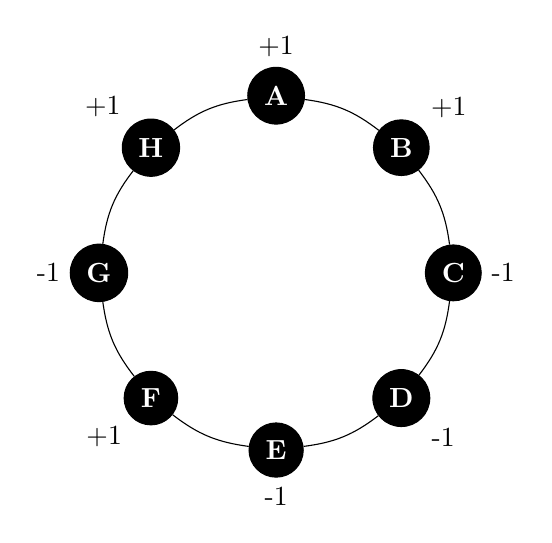
\begin{tikzpicture}[x=1.5cm, y=1.5cm, baseline={(current bounding box.north)}]
\node[draw, circle, fill=black, text=white, label={0:-1}] (C) at (1.5, 0) {\textbf{C}};
\node[draw, circle, fill=black, text=white, label={45:+1}] (B) at (1.06, 1.06) {\textbf{B}};
\node[draw, circle, fill=black, text=white, label={90:+1}] (A) at (0,1.5) {\textbf{A}};
\node[draw, circle, fill=black, text=white, label={135:+1}] (H) at (-1.06, 1.06) {\textbf{H}};
\node[draw, circle, fill=black, text=white, label={180:-1}] (G) at (-1.5, 0) {\textbf{G}};
\node[draw, circle, fill=black, text=white, label={225:+1}] (F) at (-1.06, -1.06) {\textbf{F}};
\node[draw, circle, fill=black, text=white, label={270:-1}] (E) at (0, -1.5) {\textbf{E}};
\node[draw, circle, fill=black, text=white, label={315:-1}] (D) at (1.06, -1.06) {\textbf{D}};
\path[-] (A) edge [bend left=15] (B);
\path[-] (B) edge [bend left=15] (C);
\path[-] (C) edge [bend left=15] (D);
\path[-] (D) edge [bend left=15] (E);
\path[-] (E) edge [bend left=15] (F);
\path[-] (F) edge [bend left=15] (G);
\path[-] (G) edge [bend left=15] (H);
\path[-] (H) edge [bend left=15] (A);
\end{tikzpicture} \\

Interestingly, it turns out that no matter which $n$ points are labeled $+1$ and which $n$ points are labeled $-1$,
there is always at least one point you can start at to win the game. \\

Prove, by induction, that the above fact is true for any $n \ge 1$. \\

\annotate{Check the Guide to Induction and Inductive Proofwriting Checklist before starting this one. In particular, what's the quantifier in the statement we're trying to prove? Based on that, should we be trying to ``build up'' (take a smaller game and add nodes) or ``build down'' (take a larger game and remove nodes)?}

\begin{shaded}
Provide a proof here.
\end{shaded}

\pagebreak

\section{Nim}

\emph{Nim} is a family of games played by two players. The game begins with several piles of stones, each of which has zero or more stones in it, shared between the two players. Players alternate taking turns removing any nonzero number of stones from any single pile of their choice. If at the start of a player's turn all the piles are empty, then that player loses the game. \\

Prove, by induction, that if the game is played with just two piles of stones, each of which begins with exactly the same number of stones, then the second player can always win the game if she plays correctly. \\

\annotate{Play this game with a partner until you can find a winning strategy. Once you spot the pattern, see if you can find a way to formalize it using induction. Be wary of writing statements of the form ``and so on'' or ``by repeating this;'' those aren't rigorous ways to formalize that a process will eventually do something.}

\begin{shaded}
Provide a proof here.
\end{shaded}

\pagebreak

\section{Independent and Dominating Sets}

An \emph{independent set} in a graph $G = (V, E)$ is a set $I \subseteq V$ with
the following property:
$$
  \forall u \in I.\ \forall v \in I.\ \{u, v\} \not\in E.
$$
Let's begin with a quick warm-up about independent sets.

\begin{enumerate}[label=\roman*.,ref=\roman*,topsep=0pt]
  \item Consider the graph shown below. Give two different independent sets of
    this graph, each of which has cardinality three or greater. No
    justification is necessary.

    \begin{center}
    \begin{minipage}{0.5\textwidth}
    \tikzset{every state/.style={inner sep=6pt,minimum size=0pt}}
    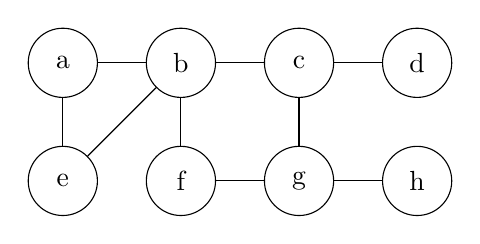
\begin{tikzpicture}[node distance=1.5cm,on grid,auto,
        baseline={(current bounding box.north)}]
      \node[state] (a) {a};
      \node[state] (b) [right=of a] {b};
      \node[state] (c) [right=of b] {c};
      \node[state] (d) [right=of c] {d};
      \node[state] (e) [below=of a] {e};
      \node[state] (f) [below=of b] {f};
      \node[state] (g) [below=of c] {g};
      \node[state] (h) [below=of d] {h};
      \path[-]
        (a) edge node {} (b)
        (a) edge node {} (e)
        (b) edge node {} (c)
        (b) edge node {} (e)
        (b) edge node {} (f)
        (c) edge node {} (d)
        (c) edge node {} (g)
        (f) edge node {} (g)
        (g) edge node {} (h);
    \end{tikzpicture}
    \end{minipage}
    \end{center}

    \begin{shaded}
      Write your answer here.
    \end{shaded}
\end{enumerate}

Now, a new definition. A \emph{dominating set} in $G$ is a set $D \subseteq V$
with the following property:
$$
  \forall v \in V.\ (v \not\in D \rightarrow \exists u \in D.\ \{u, v\} \in E).
$$
As above, it's good to play around with this definition a bit before moving on.

\begin{enumerate}[resume*]
  \item Give two different examples of dominating sets of the above graph, each
    of which has cardinality four or less. No justification is necessary.
    \begin{shaded}
      Write your answer here.
    \end{shaded}

  \item Let $G = (V, E)$ be a graph with the following property: every node in
    G is adjacent to at least one other node in $G$. Prove that if $I$ is an
    independent set in $G$, then $V - I$ is a dominating set in $G$.

    \annotate{Notice that we're asking you to show that $V - I$ is a dominating
      set, not that $I$ is a dominating set. Also, we recommend drawing some
      pictures here to get a sense of how this works. After all, you have a
      couple of examples of independent sets from part (i) of this problem!}

    \annotate{Use the formal definitions to guide your proofs. If you proceed
      via a direct proof or via contrapositive, what, exactly, will you be
      assuming, and what will you be proving? If you write this as a proof by
      contradiction, what specifically is it that you're assuming for the sake
      of contradiction?}

    \begin{shaded}
      Provide a proof here.
    \end{shaded}
\end{enumerate}

An independent set $I$ in a graph $G$ is a \emph{maximal independent set} in
$G$ if there is no independent set $I'$ in $G$ where $I \subsetneq I'$. (Here,
$I \subsetneq I'$ denotes that $I$ is a strict subset of $I'$).

\begin{enumerate}[resume*]
  \item Find independent sets $I$ and $J$ of the graph from part (i) of this
    problem such that $I$ is maximal but $\abs{I} < \abs{J}$. No justification
    is necessary.

    \annotate{Yes, this is possible. The definition of a maximal independent
      set is meant to be taken literally.}

    \begin{shaded}
      Write your answer here.
    \end{shaded}

  \item Prove that if $I$ is a maximal independent set in $G = (V, E)$, then
    $I$ is a dominating set of $G$.

    \annotate{You can build a great intuition for this result by drawing some
      pictures and thinking about what has to happen for a set of nodes to be
      an independent set and for a set of nodes to be a dominating set. When it
      comes time to write out your proof, however, you'll need to use the
      formal first-order definitions of independent sets, maximal independent
      sets, and dominating sets.}

    \begin{shaded}
      Provide a proof here.
    \end{shaded}
\end{enumerate}

\pagebreak


\section{Bipartite Graphs}

There are a few famous families of graphs that come up over and over again. One of the most important types of graphs in computer science is the \textit{bipartite graph}, which is the focus of this problem. \\

Let's begin with a formal definition of bipartite graphs. An undirected graph $G = (V, E)$ is called \emph{bipartite} if there exists two sets $V_1$ and $V_2$ such that
\begin{itemize}
\item every node $v \in V$ belongs to exactly one of $V_1$ and $V_2$,
and
\item every edge $e \in E$ has one endpoint in $V_1$ and the other in $V_2$.
\end{itemize}

The sets $V_1$ and $V_2$ here are called the \textit{\textbf{bipartite classes}} of $G$. To help you get a better sense for why bipartite graphs are important and where they show up, let's work through a couple of examples. 

\begin{enumerate}[label=\roman*]
    \item Consider a graph where each node represents a square on a chessboard and where there's an edge between any pair of squares that are immediately adjacent in one of the four cardinal directions (up, down, left, and right). Explain why this is a bipartite graph by telling us what the bipartite classes are and briefly explaining why all the edges have one endpoint in each bipartite class.

    \annotate{Draw lots of pictures!}
    
    \begin{shaded}
    Write your answer here.
    \end{shaded}
\end{enumerate}

Bipartite graphs have many interesting properties. One of the most fundamental is this one:
\begin{center}
\emph{Theorem:} An undirected graph is bipartite if and only if it contains no cycles of odd length.
\end{center}

The forward direction of this implication has a nice intuition.

\begin{enumerate}[resume*]
    \item Explain, intuitively, why if $G$ is bipartite, then it has no cycles of odd length. Specifically, give us a brief, informal explanation as to why every cycle in $G$ has to have even length.
    
    \begin{shaded}
    Write your answer here.
    \end{shaded}
\end{enumerate}

The reverse direction of this implication -- that if $G$ has no cycles of odd length, then $G$ is bipartite -- requires a different sort of argument. \\

Let's pick some arbitrary graph $G = (V, E)$ that has no cycles of odd length. For simplicity's sake, we'll assume that $G$ has just one connected component. If $G$ has two or more connected components, we can essentially treat each one of them as individual graphs. \textit{(Do you see why?)} \\

Now, choose any node $v \in V$. Using node $v$ as an ``anchor point,'' we can define two sets $V_1$ and $V_2$ that we'll need for the remainder of this argument:
\begin{gather*}
V_1 = \{ x \in V \mid \text{there is an odd-length path from $v$ to $x$} \} \\
V_2 = \{ x \in V \mid \text{there is an even-length path from $v$ to $x$} \}
\end{gather*}
This turns out to be a really useful way to group the nodes of $G$.

\begin{enumerate}[resume*]
\item Given the choices of $G$ and $v$ from above, prove that $V_1$ and $V_2$ have no nodes in common.

\annotate{Remember that there might be multiple different paths of 
different lengths from v to some other node x, so
be careful not to talk about ``the'' path between v and x. Also note that these \emph{do not} have to be \emph{simple} paths.}

\begin{shaded}
Provide a proof here.
\end{shaded}

\item Using your result from part (iii), prove that $G$ is bipartite.

\annotate{The most common mistake on this problem is to not address all the parts of the definition of a bipartite graph. So start off by writing down a list of what you need to prove, then address each part in turn.}

\begin{shaded}
Provide a proof here.
\end{shaded}

\end{enumerate}

\pagebreak
















\section{Constructing DFAs}

For each of the following languages over the indicated alphabets, construct a DFA that accepts precisely the strings that are in the indicated language. Your DFA does not have to have the fewest number of states possible, though for your own edification we'd recommend trying to construct the smallest DFAs possible. \\

\emph{Please use our online tool to design, test, and submit your answers to this problem. Handwritten or typed solutions will not be accepted.} To use the tool, visit the CS103 website and click the ``DFA/NFA Editor'' link under the ``Resources'' header. If you submit in a pair, in your GradeScope submission, let us know the SUNetID (e.g. htiek, but not 06001234) of the partner who submitted the DFAs. \\

Unlike the programming assignments, you will not be able to see the results of the autograder when you submit. As a result, \emph{be sure to test your solutions thoroughly before you submit!}

\begin{enumerate}[label*=\roman*.,ref=\roman*]
    \item 
    \begin{minipage}[t]{.55\textwidth}
    There are many ways to tile a $2 \times 8$ checkerboard with dominoes, two of which are shown to the right. Notice that the horizontal dominoes must appear as stacked pairs (do you see why?) We can read each tiling from left to right as a string made from the characters \ttt{I} and \ttt{B}, where \ttt{I} denotes ``a vertical domino'' and \ttt{B} denotes ``two horizontal dominoes.'' The top tiling here would be represented as \ttt{BIBIII} and the bottom tiling as \ttt{IBBBI}.
    \end{minipage}
    \quad
    \begin{minipage}[t]{.4\textwidth}
    \tikzset{
        rect white/.style={draw, fill=white},
        rect gray/.style={draw, fill=black!20},
        rect blue/.style={draw=none, fill=blue!40},
    }
    \begin{tikzpicture}[scale=0.7,baseline={(current bounding box.north)}]
        \draw[rect white] (0,0) rectangle (1,1);
        \draw[rect gray] (1,0) rectangle (2,1);
        \draw[rect white] (2,0) rectangle (3,1);
        \draw[rect gray] (3,0) rectangle (4,1);
        \draw[rect white] (4,0) rectangle (5,1);
        \draw[rect gray] (5,0) rectangle (6,1);
        \draw[rect white] (6,0) rectangle (7,1);
        \draw[rect gray] (7,0) rectangle (8,1);
        \draw[rect gray] (0,1) rectangle (1,2);
        \draw[rect white] (1,1) rectangle (2,2);
        \draw[rect gray] (2,1) rectangle (3,2);
        \draw[rect white] (3,1) rectangle (4,2);
        \draw[rect gray] (4,1) rectangle (5,2);
        \draw[rect white] (5,1) rectangle (6,2);
        \draw[rect gray] (6,1) rectangle (7,2);
        \draw[rect white] (7,1) rectangle (8,2);
        \draw[rect blue] (0.1,0.1) rectangle (1.9,0.9);
        \draw[rect blue] (0.1,1.1) rectangle (1.9,1.9);
        \draw[rect blue] (2.1,0.1) rectangle (2.9,1.9);
        \draw[rect blue] (3.1,0.1) rectangle (4.9,0.9);
        \draw[rect blue] (3.1,1.1) rectangle (4.9,1.9);
        \draw[rect blue] (5.1,0.1) rectangle (5.9,1.9);
        \draw[rect blue] (6.1,0.1) rectangle (6.9,1.9);
        \draw[rect blue] (7.1,0.1) rectangle (7.9,1.9);
    \end{tikzpicture} \\
    
    \begin{tikzpicture}[scale=0.7,baseline={(current bounding box.north)}]
        \draw[rect white] (0,0) rectangle (1,1);
        \draw[rect gray] (1,0) rectangle (2,1);
        \draw[rect white] (2,0) rectangle (3,1);
        \draw[rect gray] (3,0) rectangle (4,1);
        \draw[rect white] (4,0) rectangle (5,1);
        \draw[rect gray] (5,0) rectangle (6,1);
        \draw[rect white] (6,0) rectangle (7,1);
        \draw[rect gray] (7,0) rectangle (8,1);
        \draw[rect gray] (0,1) rectangle (1,2);
        \draw[rect white] (1,1) rectangle (2,2);
        \draw[rect gray] (2,1) rectangle (3,2);
        \draw[rect white] (3,1) rectangle (4,2);
        \draw[rect gray] (4,1) rectangle (5,2);
        \draw[rect white] (5,1) rectangle (6,2);
        \draw[rect gray] (6,1) rectangle (7,2);
        \draw[rect white] (7,1) rectangle (8,2);
        \draw[rect blue] (0.1,0.1) rectangle (0.9,1.9);
        \draw[rect blue] (1.1,0.1) rectangle (2.9,0.9);
        \draw[rect blue] (1.1,1.1) rectangle (2.9,1.9);
        \draw[rect blue] (3.1,0.1) rectangle (4.9,0.9);
        \draw[rect blue] (3.1,1.1) rectangle (4.9,1.9);
        \draw[rect blue] (5.1,0.1) rectangle (6.9,0.9);
        \draw[rect blue] (5.1,1.1) rectangle (6.9,1.9);
        \draw[rect blue] (7.1,0.1) rectangle (7.9,1.9);
    \end{tikzpicture}
    \end{minipage}

    Let $\Sigma$ be the alphabet $\{\ttt{B}, \ttt{I}\}$. Construct a DFA for the language $\{ w \in \Sigma^* \mid w$ represents a domino tiling of a $2 \times 8$ checkerboard\}.
    
    \item You're taking a walk with your dog along a straight-line path. Your dog is on a leash of length two, so the distance between you and your dog can be at most two units. You and your dog start at the same position. Consider the alphabet $\Sigma = \{\ttt{y}, \ttt{d}\}$. A string in $\Sigma^*$ can be thought of as a series of events in which either you or your dog moves forward one unit. For example, the string \ttt{yydd} means you take two steps forward, then your dog takes two steps forward.
    
    Let $L$ be the language $\{ w \in \Sigma^* \mid w$ describes a series of steps where you and your dog are never more than two units apart\}. Construct a DFA for $L$.
    
    \item Let $\Sigma = \{\ttt{a}, \ttt{b}, \ttt{c}, \ldots, \ttt{z}\}$. Construct a DFA for the language $\{ w \in \Sigma^*\ |\ w$ contains the word \ttt{cocoa} as a substring\}. For example, $\ttt{mm\match{cocoa}mm} \in L$ and $\ttt{\match{cocoa}} \in L$, but $\ttt{c} \notin L$, $\ttt{chocolate} \notin L$ (though \ttt{cocoa} is a sub\emph{sequence} of \ttt{\match{c}h\match{oco}l\match{a}te}. it's not a sub\emph{string}), and $\epsilon \notin L$
    
    Fun fact: DFAs and their variants are often used in string-processing algorithms and data structures. Take CS166 for more details!

    \annotate{Test your automaton thoroughly. This one has some tricky edge cases.}

\end{enumerate}

\begin{shaded}
Write the SUNetID of the person who submitted the DFAs here. 
\end{shaded}

\pagebreak

\section{Constructing NFAs}

For each of the following languages over the indicated alphabets, construct an NFA that accepts precisely the strings that are in the indicated language. \emph{Please use our online system to design, test, and submit your automata}; see above for details. As before, \emph{please test your submissions thoroughly!}

As before, while you don't have to submit the smallest NFAs possible, we recommend that you try to keep your NFAs small both to make testing easier and for your own edification.

\begin{enumerate}[label*=\roman*.,ref=\roman*]
    \item For the alphabet $\Sigma = \{\ttt{a}, \ttt{b}, \ttt{c}\}$, construct an NFA for the language $\{ w \in \Sigma^* \mid w$ ends in \ttt{a}, \ttt{bb}, or \ttt{ccc} \}.
    
    \annotate{While it's possible to do this completely deterministically, it's a bit easier if you use the ``guess-and-check'' framework we talked about in class.}

    \item For the alphabet $\Sigma = \{\ttt{a}, \ttt{b}, \ttt{c}, \ttt{d}, \ttt{e}\}$, construct an NFA for the language $\{ w \in \Sigma^*\ |$ the last character of $w$ appears nowhere else in $w$, and $|w| \ge 1 \}$. 
    
    \annotate{This problem is all about embracing nondeterminism. Use the ``guess-and-check'' framework. What information would you want to guess? How would you check it? Please don't try to solve this problem by building a DFA for this language; you'll need at least 50 states if you try to approach things this way.}
    
    \annotate{Stuck? Try reducing the alphabet to two or three letters and see if you can solve that version.}

    \item For the alphabet $\Sigma = \{\ttt{a}, \ttt{b}\}$, construct an NFA for the language $\{w \in \Sigma^* \mid w$ contains at least two \ttt{b}'s with exactly five characters between them\}. For example, \ttt{\underline{b}aaaaa\underline{b}} is in the language, as is \ttt{aabaa\underline{b}aaabb\underline{b}} and \ttt{a\underline{b}bbbba\underline{b}aaaaaaab}, but \ttt{bbbbb} is not, nor are \ttt{bbbab} or \ttt{aaabab}.
    
    \annotate{The smallest DFA for this language is pretty big, so please don't solve this one deterministically. Embrace the nondeterminism! What would you like to guess? How would you check that your guess is right?}

\end{enumerate}

\begin{shaded}
Write the SUNetID of the person who submitted the NFAs here. 
\end{shaded}

\pagebreak

\section{Designing Regular Expressions}

Below are a list of alphabets and languages over those alphabets. For each language, write a regular expression for that language. \emph{Please use our online tool to design, test, and submit your regular expressions. Typed or handwritten solutions will not be accepted.} To use it, visit the CS103 website and click the ``Regex Editor'' link under the ``Resources'' header. If you submit in a pair, please tell us in your GradeScope submission who submitted your answers to this question. Also, as a reminder, please test your submissions thoroughly, since we'll be grading them with an autograder.

\begin{enumerate}[label*=\roman*.,ref=\roman*]
    \item Let $\Sigma = \{\ttt{a}, \ttt{b}, \ttt{c}, \ttt{d}, \ttt{e}\}$. Write a regular expression for the language $\{w \in \Sigma^* \mid $ the letters in $w$ are sorted alphabetically\}. 
    
    \annotate{Note that strings in this language could be just a single character such as \ttt{a}, \ttt{b}, \ttt{c}, and could also contain repeated letters such as \ttt{aaaabbbcc}.}
    
    \item Write a regular expression for the complement of the language from part (i) of this problem.
    
    \annotate{As with NFAs, there's no simple way to start with a regex for a language $L$ and to turn it into a regex for $\overline{L}$.}
    
    \item On Unix-style operating systems like macOS or Linux, files are organized into directories. You can reference a file by giving a \textit{path} to the file, a series of directory names separated by slashes. For example, the path \ttt{/home/username/} might represent a user's home directory, and a path like \ttt{/home/username/Documents/PS5.tex} might represent that person's solution to this problem set. Paths that start with a slash character are called \textit{absolute paths} and say exactly where the file is on disk. Paths that don't start with a slash are called \textit{relative paths} and say where, relative to the current folder, a file can be found. For example, if I'm logged into my computer and am in my home folder, I could look up the file \ttt{Documents/PS5.tex} to find my solution to this problem set.
    
    The general pattern here is that a file path consists of a series of directory or file names separated by slashes. That path might optionally start with a slash, but isn't required to, and it might option- ally end with a slash, but isn't required to. However, you can't have two consecutive slashes. \footnote{In some cases you technically \textit{can} have multiple consecutive slashes, but we'll ignore that for now.}
    
    Let $\Sigma = \{a,/\}$. Write a regular expression for $L = \{w \in \Sigma^* \mid w$ represents the name of a file path on a Unix-style system \}. For example, $\ttt{/aaa/a/aa} \in L$, $\ttt{/} \in L$, $\ttt{a} \in L$, $\ttt{/a/a/a/} \in L$, and $\ttt{aaa/} \in L$, but $\ttt{//a//} \notin L$, $\ttt{a//a} \notin L$, and $\varepsilon \notin L$.
    
    Fun fact: this problem comes from my job, where I fixed a bug in industrial code that arose when someone wrote the wrong regex for this language. 
    
    \item Suppose you are taking a walk with your dog on a leash of length two. Let $\Sigma = \{\ttt{y}, \ttt{d}\}$ and let  $L = \{w \in \Sigma^* \mid w$ represents a walk with your dog on a leash where you and your dog both end up at the same location\}. For example, we have $\ttt{yyddddyy} \in L$ because you and your dog are never more than two steps apart and both of you end up four steps ahead of where you started; similarly, $\ttt{ddydyy} \in L$. However, $\ttt{yyyyddd} \notin L$, since halfway through your walk you're three steps ahead of your dog; $\ttt{ddyd} \notin L$, because your dog ends up two steps ahead of you; and $\ttt{ddyddyyy} \notin L$, because at one point your dog is three steps ahead of you. Write a regular expression for $L$.
    
    \annotate{Note that, unlike in Problem 1, you and your dog \textbf{must} end at the same position.}
    
\end{enumerate}
\begin{shaded}
Write the SUNetID of the person who submitted the regular expressions here. 
\end{shaded}

\pagebreak

\section{Finite Languages}

A language $L$ is called \emph{finite} if $L$ contains finitely many strings (that is, $|L|$ is a natural number). \\

Given a finite language $L$, explain how to write a regular expression for $L$. Briefly justify your answer; no formal proof is necessary. This shows that all finite languages are regular. \\
    
\annotate{Watch for edge cases!}
    
\begin{shaded}
Write your answer here.
\end{shaded}

\pagebreak

\section{Monoids and Kleene Stars}

The Kleene star operator is one of the more unusual operators we've covered over the course of the quarter. This problem explores one of its fundamental properties. \\

Let $\Sigma$ be an arbitrary alphabet. A \emph{monoid over $\mathbf{\Sigma}$} is a set $M \subseteq \Sigma^*$ with the following properties:
\begin{equation*}
\varepsilon \in M \quad\quad\quad \forall x \in M.\ \forall y \in M.\ xy \in M.
\end{equation*}

Let $L$ be an arbitrary language over $\Sigma$ and let $M$ be an arbitrary monoid over $\Sigma$. Prove by induction that if $L \subseteq M$, then $L^* \subseteq M$. In the course of writing this proof, please call back to the formal definition of language concatenation and the Kleene star. Here's a refresher on the definitions:
    \begin{align*}
    L_1L_2 &= \{ wx\ |\ w \in L_1\text{ and }x \in L_2 \} \\
    L^0 &= \{\varepsilon\} \quad\quad\quad L^{n+1} = LL^n \\
    L^* &= \{ w\ |\ \exists n \in \N.\ w \in L^n \}
    \end{align*}
    
\annotate{To get yourself acquainted with monoids, try giving three examples of monoids. At least one of them
should be finite, and at least one of them should be infinite.} \\

\annotate{This problem is all about finding the right way to formalize things. Think about, ultimately, what it is that
you need to prove. Before you start trying to prove that, break the task down into smaller pieces and make
sure you organize everything in a way that makes the logical flow easy to read and rigorously covers all
cases. Once you have the setup put together, dive in and fill out each section.} \\
    
\annotate{If you'd like to use any properties of Kleene stars, language concatenation, etc. that aren't given in the definition, you'll need to prove them first.} \\

\begin{shaded}
Provide a proof here. 
\end{shaded}

The result that you've shown here is a building block toward a larger result: If $L$ is a language over $\Sigma$, then $L^*$ is the smallest monoid over $\Sigma$ that contains $L$.
This is a very different way of thinking about the Kleene star. Rather than talking about $L^*$ in terms of powers of languages, we can think of $L^*$ as ``what set do you get if you start with $L$ and add as little as possible to make it contain $\epsilon$ and be closed under concatenation?'' That's quite a departure from where we started! \\

The monoids we explored in this problem are actually a special case of a broader class of objects (what we've been calling ``monoids'' are actually ``concatenative monoids,'' since they focus on string concatenation). The more general version of monoids shows up in parallel programming (most famously, in MapReduce) as a way of describing what sorts of computational jobs can be split apart and joined back together later on, as well as in programming language theory as a way of capturing the notion of ``computation with side effects.'' 

\newpage


\section{DFAs, Formally}
When we first talked about graphs, we saw them first as pictures (objects connected by lines), then formally defined a graph $G$ as an ordered pair $(V, E)$, where $V$ is a set of nodes and $E$ is a set of edges. This rigorous definition tells us what a graph actually is in a mathematical sense, rather than just what it looks like. \\

We've been talking about DFAs for a while now and seen how to draw them both as a collection of states with transitions (that is, as a state-transition diagram) and as a table with rows for states and columns for characters. But what exactly \textit{is} a DFA, in a mathematical sense? \\

Formally speaking, a DFA is a 5-tuple $(Q, \Sigma, \delta, q_0, F)$, where
\begin{itemize}
    \item $Q$ is a finite set, the elements of which we call \textit{states};
    \item $\Sigma$ is a finite, nonempty set, the elements of which we call \textit{characters};
    \item $\delta\ :\ Q \times \Sigma \rightarrow Q$ is the \emph{transition function}, described below;
    \item $q_0 \in Q$ is the start state;
    \item $F \subseteq Q$ is the set of accepting states.
\end{itemize}
The transition function warrants a bit of explanation. When we've drawn DFAs, we've represented the transitions either by arrows labeled with characters or as a table with rows and columns corresponding to states and symbols, respectively. In this formal definition, the transition function $\delta$ is what ultimately specifies the transition (the $\delta$ symbol is a Greek lower-case delta). \\

First, let's talk about the domain and codomain of this function. We're introducing some new notation when we say the domain of this function is $Q \times \Sigma$. If $A$ and $B$ are sets, the \textbf{\textit{Cartesian product}} of $A$ and $B$, denoted $\mathbf{A \times B}$,
is the set
\begin{equation*}
\{ (x, y)\ |\ x \in A \land y \in B \}
\end{equation*}
Intuitively, $A \times B$ is the set of all ordered pairs you can make by taking one element from $A$ and one element
from $B$, in that order. For example, the set $\{\textcolor{red}{1}, \textcolor{red}{2}\} \times \{\textcolor{blue}{u}, \textcolor{blue}{v}, \textcolor{blue}{w}\}$ is
\begin{equation*}
\{\ (\textcolor{red}{1}, \textcolor{blue}{u}), (\textcolor{red}{1}, \textcolor{blue}{v}), (\textcolor{red}{1}, \textcolor{blue}{w}), (\textcolor{red}{2}, \textcolor{blue}{u}), (\textcolor{red}{2}, \textcolor{blue}{v}), (\textcolor{red}{2}, \textcolor{blue}{w})\ \}
\end{equation*}

Thus, the input to our function will be an ordered pair of the form $(q, a)$ where $q \in Q$ and $a \in \Sigma$. Then the transition from state $q$ on symbol $a$ is given by $\delta(q, a)$, which produces an element in our codomain $Q$ representing the state we should transition to from $q$ upon reading $a$. \\

This question explores some properties of this rigorous definition.

\begin{enumerate}[label*=\roman*.,ref=\roman*]
    \item Is it possible for a DFA to have no states? If so, define a DFA with no states as a 5-tuple, explaining why your 5-tuple meets the above requirements. If not, explain why not.
    
    \annotate{To define an object using a 5-tuple, use this template: ``Let $D = (Q, \Sigma, \delta, q_0, F)$, where $Q = \dots, \Sigma = \dots$,'' etc. Defining a DFA requires you to define a transition function $\delta$. To help you see how our study of functions this quarter applies here, we'd like you to formally define $\delta$ either using a fixed rule or as a piecewise function. For the purposes of this problem, please \textbf{do not} give a picture or table for $\delta$, even though in general these could be valid ways of describing a function. If you've having trouble doing so, it might mean that you picked too complex of a DFA and might want to search for something simpler.}
    
    \begin{shaded}
    Write your answer here.
    \end{shaded}
    
    \item Is it possible for a DFA to have no \textit{accepting} states? If so, define a DFA with no accepting states as a 5-tuple, explaining why your 5-tuple meets the above requirements. If not, explain why not.
    
    \begin{shaded}
    Write your answer here.
    \end{shaded}
    
    \item In class, we said that a DFA must obey the rule that for any state and any symbol, there has to be exactly one transition defined on that symbol. What part of the above definition guarantees this?
    
    \begin{shaded}
    Write your answer here.
    \end{shaded}
    
    \item Is it possible for a DFA to have an unreachable state (that is, a state that is never entered regardless of what string you run the DFA on)? If so, define a DFA with an unreachable state as a 5-tuple, explaining why your 5-tuple meets the above requirements. If not, explain why not.
    
    \begin{shaded}
    Write your answer here.
    \end{shaded}
\end{enumerate}

\pagebreak 

We've included several optional fun problems here. Feel free to work on any number of them, but please submit at most one of them with your problem set. If you submit more than one problem, we'll select which one to grade arbitrarily and capriciously. \smiley

\section*{Optional Fun Problem One: Why Finite? (Extra Credit)}

We'll say that a \emph{deterministic infinite automaton}, or \emph{DIA}, is a generalization of a DFA in which the automaton has infinitely many different states. Formally speaking, a DIA is given by the same 5-tuple definition as a DFA from Problem Nine, except that $Q$ must be an infinite set. Since DIAs have infinitely many states, ther're mostly an object of purely theoretical study. You couldn't actually build one in the real world. \\

Prove that if $L$ is an arbitrary language over an alphabet $\Sigma$, then there is a DIA that accepts $L$ (that is, the DIA accepts every string in $L$ and rejects every string not in $L$.) To do so, show how to start with a language $L$, formally define a 5-tuple corresponding to a DIA for $L$, then formally prove that that DIA accepts all and only the strings in $L$.

\begin{shaded}
Write your answer and proof here. 
\end{shaded}

\section*{Optional Fun Problem Two: Edit Distances (Extra Credit)}

The \emph{edit distance} between two strings $w$ and $x$ is the minimum number of edits that need to be made to $w$ to convert it into $x$. Here, an \emph{edit} consists of either adding a character somewhere into $w$, deleting a character
somewhere from $w$, or replacing a character of $w$ with another. For example, \ttt{cat} and \ttt{dog} have edit
distance 3, \ttt{table} and \ttt{maple} have edit distance 2, and \ttt{edit} and \ttt{distance} have edit distance 6. \\

Let $\Sigma = \{\ttt{w}, \ttt{h}, \ttt{i}, \ttt{m}, \ttt{s}, \ttt{y}\}$. Design an NFA for $\{w \in \Sigma^* \mid$ the edit distance of $w$ and \ttt{whimsy} is at most
three\}. Submit your answer online, and let us know in your written assignment who made the submission.

\begin{shaded}
Write the SUNetID of the person who submitted the NFA here. 
\end{shaded}
































\section*{Optional Fun Problem Three: Egyptian Fractions (Extra Credit)}

The Fibonacci sequence mentioned in Problem One is named after Leonardo Fibonacci, an eleventh-century Italian mathematician who is credited with introducing Hindu-Arabic numerals (the number system we use today) to Europe in his book \textit{Liber Abaci}. This book also contained an early description of the Fibonacci sequence, from which the sequence takes its name. \textit{Liber Abaci} also described a method of writing out fractions called \emph{Egyptian fractions}, which has been employed since ancient times; the Rhind Mathematical Papyrus, composed about 3,500 years ago in Thebes, includes several tables of fractions written out this way. \\

An Egyptian fraction is a sum of \emph{distinct} fractions whose numerators are all one (these fractions are called \textit{unit fractions}). For example, here are several Egyptian fraction representations of rational numbers:
\begin{alignat*}{3}
& \frac{2}{3} = \frac{1}{2} + \frac{1}{6} \qquad\qquad\qquad && \frac{2}{15} = \frac{1}{10} + \frac{1}{30} \\
& \frac{7}{15} = \frac{1}{3} + \frac{1}{8} + \frac{1}{120} && \frac{2}{85} = \frac{1}{51} + \frac{1}{255}
\end{alignat*}

Egyptian fractions are useful for divvying up objects fairly. For example, suppose you have two cakes to distribute to fifteen people -- that is, everyone should get a $\frac{2}{15}$ fraction of those cakes. Begin by slicing each cake into tenths and giving each person one ($\frac{1}{10}$). Now, take the remaining tenths you haven't distributed and cut them into thirds, giving thirtieths of the original cake. Each person then takes one of those ($\frac{1}{30}$). Because $\frac{1}{10} + \frac{1}{30} = \frac{2}{15}$, everyone gets their fair share. Pretty cool, isn't it? \\

One way of finding an Egyptian fraction representation of a rational number is to use a \textit{greedy algorithm} that works by finding the largest unit fraction at any point that can be subtracted out from the rational number. For example, to compute the fraction for $\frac{42}{137}$, we would start off by noting that $\frac{1}{4}$ is the largest unit fraction less than $\frac{42}{137}$. We then say that
$$\frac{42}{137} = \frac{1}{4} + \left(\frac{42}{137} - \frac{1}{4}\right) = \frac{1}{4} + \frac{31}{548}$$
We then repeat this process by finding the largest unit fraction less than $\frac{31}{548}$ and subtracting it out. This number is $\frac{1}{18}$, so we get
$$\frac{42}{137} = \frac{1}{4} + \left(\frac{42}{137} - \frac{1}{4}\right) = \frac{1}{4} + \frac{1}{18} + \left(\frac{31}{548} - \frac{1}{18}\right) = \frac{1}{4} + \frac{1}{18} + \frac{5}{4,932}$$
The largest unit fraction we can subtract from $\frac{5}{4,932}$ is $\frac{1}{987}$:
$$\frac{42}{137} = \frac{1}{4} + \frac{1}{18} + \frac{1}{987} + \left(\frac{5}{4,932} - \frac{1}{987}\right) = \frac{1}{4} + \frac{1}{18} + \frac{1}{987} + \frac{1}{1,622,628}$$
And at this point we're done, because the leftover fraction is itself a unit fraction. \\

Prove that the greedy algorithm for Egyptian fractions always terminates for any rational number $r$ in the range $0 < r < 1$ and always produces a valid Egyptian fraction. (A \emph{rational number} is a real number that can be written as $r = \frac{p}{q}$ for some integers $p$ and $q$ where $q \neq 0$.) That is, the sum of the unit fractions should be the original number, and no unit fraction should be repeated. This shows that every rational number in the range $0 < r < 1$ has at least one Egyptian fraction representation.
\begin{shaded}
Provide a proof here.
\end{shaded}

\end{document}